\section{A Survey of Semantic Desktops}
\label{sec:sd}

We have covered so far the futuristic systems of the past and the visionaries who imagined them, like the Memex, which since 1945 have been an inspiration for most of the work in personal computing and personal information management. We have also briefly described the Semantic Web and its technologies. We will now show through a list of “modern” Semantic Desktops how semantic technologies are put to use in those systems to realise the vision of the Memex, and more.

\subsection{Common Challenges}
\label{sec:sdgoals}

The term \emph{Semantic Desktop} was coined in 2003 by Decker and Frank and was taken up first by Sauermann in Gnowsis \cite{Sauermann2003}. 

The [Social] Semantic Desktop saw the fastest rise and uptake during the 2004 -- 2009 period, when most research work was put into the development of systems and applications, new and improved algorithms to support knowledge work. 
These systems and tools were aiming to solve similar problems as was the Memex before them: supporting and improving knowledge work by mimicking the way the brain works --- using Bush's associative trails reworked with the help of the semantic technologies. 
The fast growth of the digital world, while providing easier access to information and communication, has created new problems, foreseen by Nelson in the 70s: there is so much information available that it becomes unmanageable. 

Thus, the challenges that the Semantic Desktops aim to solve can be described as follows:
\begin{description}
 \item[Information overload] caused by the ease with which information can now be generated, shared, stored and accumulated. The amount of information that we see, receive, create every day is enormous. While the storage and processing capacity of hardware has increased many-fold, re-finding stored information has become a more complex task. The challenge is to enable users to manage this large amount of information better, while not spending more time and effort organising it. 
 \item[Data silos] are created by desktop applications which store their data in proprietary  formats, in storage inaccessible to other applications which could possibly reuse that information, thus each mus recreate it in their own formats and store it in their own walled repositories. 
 The negative effects of this vicious circle are \emph{data duplication}, and \emph{disconnected information}. Having the same data in multiple applications leads to difficulties in keeping it up to date and synchronised. Additionally, having pieces of information relating to the same object or entity spread over several locations and tools makes working with that information more difficult, as it requires opening and browsing through several folder hierarchies and application structures, as well as piecing together the information every time it is needed. The challenge presented by data silos is to give users a unified and consistent view over their data, regardless of its source and location. 
 \item[Dynamic data] means that information changes over time, and thus it can become deprecated. Using deprecated information can have undesired effects, like sending emails to an old email address of a contact. The data silos problem above adds complexity to this --- \emph{duplication of data} in various applications makes it more difficult to decide which version is correct; \emph{disconnected information} means that when a piece of information changes, care must be taken so that the changes are made in every place where the information is kept, increasing the effort required.
 \item[Associative trails] as those described by Bush, follow the way we think about things, by connections and associations, unconstrained by the way the information is stored or presented in various applications. This point is also related to the data silos issue. As we discussed above, studies showed that the way we form mental models and work with information is task and data centric. As long as data is disconnected and locked away in application repositories, explicit associative trails can only be fragmented, short and thus hurting productivity. 
\end{description}

The 2004 white paper by \cite{Decker2004} ambitiously describes a solution, the Social Semantic Desktop as ``a novel collaboration environment, enabling the creation, sharing and deployment of data and metadata'' and names the sources that would contribute to the development of such a system: ``Semantic Web, Peer-to-Peer Networks, and Online Social Networking.'' From the point of view of the future Social Semantic Desktop, the Semantic Desktop was just one piece of the puzzle, its function being that of a smart personal information management tool, that provides a common vocabulary, creates and maintains a network of interconnected personal information, stores it and gives users access to it through search and browsing.

The 2005--2006 workshop series on the Semantic Desktop, and the 2005--2008 series of hands-on workshops\footnote{\url{http://semanticweb.org/wiki/Semantic\_Desktop\#Dissemination\_activities}} served as a catalyst for early ideas and brought together researchers interested in the topic, who were already working on relevant projects. Some of the systems that are described below were introduced at these workshops: \emph{IRIS}, \emph{DeepaMehta}, \emph{HyperSD}, \emph{WonderDesk}. The workshops saw also the presentation of stand-alone semantic applications like the Semantic Clipboard \cite{Reif2006}, Beagle++ \cite{Brunkhorst2006}, Semantic Wikis \cite{Oren2005,Aumueller2005}, Semantic Instant Messaging (SAM \cite{Franz2005}, Nabu \cite{Osterfeld2005}), semantic federation \cite{Park2006}, semantic search and ranking \cite{Chirita2005}, and trust \cite{Noh2006}.

\subsection{Semantic Desktop Systems}
\label{sec:sdsystems}

In this section we present a review of existing Semantic Desktops. The NEPOMUK project is described separately in Section \ref{sub:nepomuk}. 

The Semantic Desktops presented here have the same common goals, and tackle by some extent the same challenges we described in Section \ref{sec:sdgoals}. Some of the systems cover a broad spectrum of activities, aiming for a general solution, while others are focused on precise PIM tasks like email or task management. 

We begin by describing the systems, along with their characteristics and features, and then continue by delving into the details of the architecture, services and ontologies for a subset of them. We start with the more relevant ones, which we describe in more detail. We then continue with other systems providing similar functionality. The list is ended by very specialised systems or applications, with semantic features.

\subsubsection{Haystack}

The Haystack system came out of MIT's Computer Science \& Artificial Intelligence Laboratory (CSAIL) as early as 1997. It started as a personal system for Information Retrieval, where users manage their own private information \cite{Adar1999}, and the system adapts to the users' behaviour. Although not explicitly stated, from the beginning Haystack has been a semantic system, as it created and saved metadata links, or associations between things in the user's corpus, and allowed these links to be followed from one document to another. The connections are made either by inspecting the content of the documents, or by tracking the user's activity and inferring the connections. The user can also annotate content with metadata. 

The architecture of the system evolved over time, but the overall structure remained the same \cite{Huynh2002,Quan2003b} --- a three-tiered design. At the bottom there is a storage layer for the user's content --- initially a database, later, an RDF store. On top of the storage, Haystack provided a basic data model for the objects, metadata and links; later it moved to RDF for describing the data. The RDF model is general, but it allows customisation by users \cite{Karger2006}. The top level is made of client applications which can have one of several roles: \begin{inparaenum}[(i)] \item proxies for extracting information from existing unstructured sources like user applications or the Web; \item connectors for linking already extracted information; \item observers of user actions \end{inparaenum}. There are also client services through which the user can interact directly with the data --- modify it, search it or visualise it. 

\subsubsection{Stuff I've Seen (SIS)}

The Stuff I've Seen (SIS) system is presented by \cite{Dumais2003} as a solution to re-finding previously seen information, be it in an email, on a web page or in a document. The authors recognise the problem of data loss due to ``the multiplicity of independent applications used to manage information each with its own organisational hierarchy'' and ``the limited search capabilities'' they offer. SIS was not meant to be a new PIM application, but a unified point of access to existing content from other applications. It uses a central index and provides a common search interface over existing information sources. It aids re-finding of information by employing contextual cues in the search interface. 

Developed at Microsoft, the system is based on the Microsoft Search indexing infrastructure, thus having access to functions of the operating system inaccessible to third-party applications. The architecture is modular. Five main components are chained to feed data extracted from various sources into the index. There is no mention of any semantic technologies being used, although some structured information is extracted: type of the resource, relations to other resources, like sender of an email and author of a document. The structures are then used to provide faceted query refinement. Some extraction of information from the content of the files is done with natural language processing. SIS also allows users to create metadata annotations on their content, which is an important first step towards creating semantic relations.

An extensive user evaluation of the system explored the best ways of presenting the search results, and determined which are the most common ways of searching for information. 
It found that time and people are important cues in re-finding, and thus should be included as part of the saved context. 
The importance of the time dimension is further studied in \cite{Ringel2003}, also based on the SIS system. 
Lifestreams \cite{Freeman1995,Fertig1996,Freeman2007} proposed a chronological ordering of information and a totally reworked metaphor for the desktop, based on time as a storage model. 

\subsubsection{MyLifeBits}

MyLifeBits \cite{Gemmell2002,Gemmell2003a,Bell2007} is another project by Microsoft Research, which uses the Memex as a blueprint for a digital personal store \cite{Gemmell2006}. The team behind the CyberAll project \cite{Bell2001}, which then was continued by MyLifeBits, started an ambitious task: ``to digitally store everything from one’s life, including books, articles, personal financial records, memorabilia, email, written correspondence, photos (time, location taken), telephone calls, video, television programs, and web pages visited.'' \cite{Bell2004}. The initial focus was on improving the methods for capture and storage, populating a personal ontology with digitised information from many sources. The following step was devising methods for using the information gathered --- ``tools [\dots] for annotation, collections, cluster analysis, facets for characterising the content, creation of timelines and stories'' \cite{Bell2004}.

MyLifeBits does not impose a strict single hierarchy over the user's data, but uses links and annotations to organise the objects, and collections to group them. The annotations and links play an important role in the system. In the style of Nelson's transclusion, the links are bidirectional, and serve as well to establish ownership of connected pieces of data. Annotations play several roles in the system, and are considered important especially for non-textual resources like audio, video and images, as they enable functionalities on these resources, like text search, and story-telling, which otherwise are not possible. The system includes features aiming to make annotation as easy as possible --- bulk annotation, predefined annotations, audio annotation. Collections are a special type of annotation. They are a way of supporting a loose hierarchy, without enforcing it. Overlapping collections are allowed, as well as resources which do not belong to any collection. ``Fluid'', or virtual collections are 
also supported, by saving and reusing a query.

Another important aspect of the system is the flexible visualisation it provides. A resource or a collection of resources can be presented in several ways, as different views can give different insights into the data. ``Furthermore, the visualisation must become a UI --- the user will want to click on a row of a table or a peak in a graph and see the data behind it.'' \cite{Gemmell2003a}

MyLifeBits uses a predefined schema \cite{Gemmell2006} to describe the data collected. The schema is flexible and customisable, although the authors do not anticipate that users will make many changes to it \cite{Gemmell2003a}, as this would lead to complications in using the system. There are a set of predefined types, based on common resources available on a user's desktop. Instances of these types have unique identifiers which are used to establish the relationships. Relationship between two entities are bi-directional, and the two inverse links involved must have distinct names, e.g. ``is organiser'' and ``is organised by''.

The architecture of the system is modular, with the MyLifeBits store at the centre. The store \cite{Gemmell2003a} uses a Microsoft SQL Server database to provide the schema and store the data. 

\subsubsection{Gnowsis}

Gnowsis \cite{Sauermann2003} is one of the first implementations of a Semantic Desktop which advocated the use of Semantic Web technologies on the desktop, and the creation of a ``personal Semantic Web for PIM'' \cite{Sauermann2009}. It proposes an architecture based on a local Web server as a desktop service, while integrated desktop applications communicate with it via Semantic Web protocols. In Gnowsis we encounter for the first time the notion of \emph{desktop services} in relation to the Semantic Desktop. 

Unlike Haystack, Gnowsis proposed that existing applications be modified to work with the semantic infrastructure, rather than being replaced completely. The Semantic Desktop would play the role of integration middleware by lifting semantic data from desktop formats and storing it in a central repository accessible to the applications. The extraction of data is done by adaptors, and the resulting network of semantic information can be accessed through a Web browser type of interface, which also provides access to the underlying model. 

The semantic data is described with ontologies, and the system provides a generic personal information model (PIMO) \cite{Sauermann2006}, which is rich enough to cover most use cases, but also flexible and customisable by the users. PIMO was created with the user in mind, and to support personal mental models. 

The Gnowsis Semantic Desktop largely influenced the architecture and basic design of NEPOMUK \cite{Bernardi2008}. Its main role was that of an integration system \cite{Sauermann2005a,Sauermann2005b} for knowledge management. 

\subsubsection{Integrate, Relate, Infer, Search (IRIS)}

Another Semantic Desktop system which is all about integration is IRIS (which stands for ``Integrate, Relate, Infer, Search'') \cite{Cheyer2005}. IRIS was part of  SRI's \footnote{\url{http://www.sri.com}} Cognitive Assistant that Learns and Organizes (CALO), as a personal information knowledge source \cite{Ambite2006}. It also played the role of semantic user interface, through its embedded suite of applications. 

CALO is an intelligent agent system which consists of several connected agents \cite{Ambite2005} specialised on different areas of knowledge work --- time management (PCalM \cite{Berry2004}, PTIME \cite{Berry2005a,Berry2011}, PExA \cite{Myers2007}), task management (Towel \cite{Conley2007}, PExA), contact management, and more. The AI agents are not necessarily semantic, although they do communicate with IRIS and use the semantic information it provides in their actions. CALO not only uses the knowledge, but also creates knowledge back into IRIS.

IRIS uses ontologies to describe data --- initially a comprehensive ontology was defined, but it was replaced in favour of the Component Library Specification (CLib), the ontology used in CALO. The CLib ontology is modular just like the architecture of the system --- different agents require different ontologies: there is an Office Ontology, a Meeting Ontology, a Documentation Ontology \cite{Ambite2005}.

CALO integrated parts of Personal Radar\footnote{\url{http://www.radarnetworks.com/}} into IRIS --- the triple-store implementation (Semantic Object framework), and user interface elements. One of the key features of IRIS and CALO as a whole, is the focus on machine learning. 

\subsubsection{Semantic Explorer (SEMEX)}

The Semantic Explorer (SEMEX) is another platform for semantic PIM. The system provides on-the-fly integration of personal and public data \cite{Dong2004}, by extending a user's personal information space and providing a logical view over it. SEMEX aligns the information integration task with the user's environment, making it happen as a side effect of the normal daily tasks.

The system comes with a basic domain ontology, which can be personalised by the users either by importing new models, or by manually changing it. The authors introduce the concept of malleable schemas \cite{Dong2005c}, which can be extracted from browsing patters, or even suggested by the system based on clustering of resources. Using the ontology, SEMEX extracts semantic objects from desktop sources and stores them in a central repository \cite{Dong2005a}. 
Reference reconciliation \cite{Dong2004,Dong2005b} plays an important role in the system, particularly for the on-the-fly integration. It uses background knowledge and previous mappings for integrating external sources whose schemas might not match. 

SEMEX offers an interface, similar to that of Haystack and Gnowsis, for querying and browsing by association the underlying database.

\subsubsection{Cross-COntext Semantic Information Management (X-COSIM)}

The Cross-COntext Semantic Information Management (X-COSIM) \cite{Franz2007a} is a framework which supports seamless PIM and information linkage across different contexts that users might find themselves in. 

The system provides a reference ontology called X-COSIMO. Additional to defining concepts and relations, the ontology also describes the various possible contexts and relations between the concepts and contexts. The ontology is comprehensive, therefore to simplify its use, the system offers an application development interface called X-COSIMA, aimed at developers.

The semantic functionalities are integrated into existing applications through plugins. \cite{Franz2007,Franz2009} describes and compares COSIMail and COSIFile with their non-semantically enhanced counterparts. Like other systems above, X-COSIM provides a browser for the semantic data it handles. 

\subsubsection{Multiple Ontology based Semantic DEsktop (MOSE)}

The Multiple Ontology based Semantic DEsktop (MOSE) \cite{Xiao2005} is a multi-layered ontology framework for personal information management. The user manages the data through many \emph{Personal Information Applications} (PIA) which are specialised on certain tasks, like trip planning or bibliography management. The PIAs are the main feature of MOSE \cite{Xiao2006}. They each have their own ontology to describe the domain knowledge, a user interface and a specific workflow. The PIAs can communicate and share data through mappings of their ontologies. 

MOSE stores its data in several repositories, one for the file descriptors, one for the resources and one for tracking provenance of resources to the files they were extracted from. These repositories are populated by several services of the framework, and by the PIAs. The data can be browsed by association, modified and queried through the resource explorer, a browser-like interface. Other user interfaces to the data are provided by the PIAs, which themselves can be customised or created from scratch by the users.

\subsubsection{PlacelessDocuments} 

Placeless Documents \cite{Dourish2000} offers an alternative document management architecture, based on the flexible structure created using tags, or \emph{document properties}, not the rigid hierarchy of folders. The system, created at Xerox PARC, is based on an earlier prototype called Presto \cite{Dourish1999}. It is not explicitly a ``semantic'' framework, but it has many of the features we find in the more recent Semantic Desktops: information management based on metadata, and interconnected resources. Besides using properties to organise information from documents and emails, the Placeless system is distinctive through the use of \emph{active properties}, which store executable code, and which provide services on the documents they are attached to. These ``property-based document services are centred on the document and document activity, rather than on a separate application'' thus solving the issue of application silos and allowing the user to focus on the task. Examples of such services include 
translation, summarisation, and format conversion.

The system supports generic system properties, as well as user-generated properties which enable a personalised view of the information space of the user. The properties are stored independently from the documents they describe, in a database. 

Documents can be aggregated in collections based on their properties, they can be shared and collaborated on. The framework integrates the existing storage infrastructure available, through content providers connecting to the local file system, the web, or any network-accessible repository. Placeless Documents also integrates with existing applications which can only work with classic file systems, through the NFS protocol.

\subsubsection{WonderDesk}

WonderDesk \cite{Zhang2005} is a distributed Semantic Desktop for resource management and sharing, part of WonderSpace eScience suite. It works with scientific objects, like papers, presentations, and other research artefacts. The system provides a basic vocabulary for metadata about the eScience resources and allows different domain specific vocabularies to be loaded for each scientific discipline. A separate component of WonderSpace, a P2P super-node named WonderServer, acts as an information integrator and indexer for a network of WonderDesk peers. The hybrid P2P architecture allows sharing of information between the nodes in a network, while still functioning standalone as a Semantic Desktop. It provides annotation functionalities, as well as sharing of annotations and resources within the group, and distributed querying. 

\subsubsection{HyperSD}

HyperSD \cite{Schwabe2005} is a Semantic Desktop browser which allows navigation and access to desktop resources based on metadata about them, in the style of Haystack. The application was developed with HyperDE \cite{Nunes2005,Nunes2006}, a Semantic Web application development environment. It provides wrappers for standard desktop resources like files, contacts, events, which extract the metadata and store it alongside the schema in an RDF store. The schema is simple, reusing some properties and relations from existing Web vocabularies like FOAF. 
The interface allows faceted browsing and contextual navigation, as well as creation and editing of new items or new associations. 

\subsubsection{OntoPIM} 

OntoPIM \cite{Katifori2005} is a framework for Personal Information Management that relies on the use of a Personal Ontology. It is part of a bigger project for Task-centred Information Management (TIM), and is motivated by the same challenges as described above.
OntoPIM supports storing any object of interest from the desktop, and relating it to any concept from the ontology. The Personal Ontology is just one part of the data layer of the system. There are two other ontologies, one for domain independent objects, like documents and emails; which is mapped to another one for domain specific objects; which in turn is mapped to the Personal Ontology. The users can build and modify their model through the Personal Ontology Builder and Personalisation Tool. The system provides other services on top of the semantic data --- instance matching, semantic save, querying, mapping.

\subsubsection{The Autonomic Semantic Desktop}

The Autonomic Semantic Desktop \cite{Breitman2006} introduces a semantic layer to a self-managing (or autonomic) application architecture. The result is an integrated desktop environment capable of self-managing behaviour, which uses semantics to achieve its goal of simplifying Personal Information Management, by supporting the user in maintaining their personal information in an automatic (or semi-automatic) way. The user data is extracted from two domains, the desktop and the Web \cite{Breitman2005}, and is described by a shared ontology. The data layer is used as communication interface between a set of independent pluggable services.

\subsubsection{Chandler}

Chandler \cite{ChandlerProject} is a project that defines itself as a ``Note-to-Self Organizer'', integrating personal information from multiple applications, and supporting task management and collaboration. It does not use typical Semantic Web technologies, instead it defines its own lightweight flexible vocabulary for describing the types of data, called \emph{kinds}, as well as implementing its own data storage system. However, the ideas are consistent with those of the Semantic Desktop, integrating personal information from different sources and interconnecting it for associative browsing. The system provides a single modular user interface for the data, with different views for specific data types. Collaboration and data sharing in Chandler is realised with a client-server architecture, where the server is called a \emph{hub}.

\subsubsection{SeMoDesk}

The SeMoDesk \cite{Woerndl2008} project aims to bring the Semantic Desktop to the mobile environment. It tackles the limitations of mobile devices in regard of storage, display and input, while at the same time integrating, and taking advantage of the added functionality that the devices offer, like calls, text messaging, and location \cite{Woerndl2009b}. The system uses the PIMO model defined Gnowsis and Nepomuk, for describing the data, which provides the necessary concepts for PIM. Information is extracted from the applications available on the device, like the address book, calendar, email, and task management, and from files. The architecture is also similar to the one of Gnowsis, although modified to reuse services available on the mobile platform --- the SQL database on Windows Mobile for storing the data. The user interface is adapted to the smaller screen size and the different interaction mode, by limiting the number of properties displayed based on the context of use \cite{Woerndl2009a}.

\subsubsection{MindRaider}

MindRaider \cite{MindRaider} is an open source ``Semantic Web outliner'' which aims to help organise a user's personal resources --- documents, friends, thoughts --- ``in a way that enables quick navigation, concise representation and inferencing''. The system is modelled as a mind-mapping and note-taking tool, but it allows interlinking of more types of concepts than just notes, and provides more visualisations than a mind map.
MindRaider uses existing vocabularies like FOAF, SKOS and Dublin Core in combination with custom ontologies used for classification. The data is stored in a triple store. 
It enables interoperation with Gnowsis, through a connector, which allows querying data, and reusing resources. 

\subsubsection{DeepaMehta}

DeepaMehta \cite{Richter2005} is a service oriented application framework with a data model based on topic maps. It uses visualisations guided by research from cognitive psychology, and similar to concept maps. Its main goal is to provide a user interface which follows the associative way in which the human mind operates with information, thus keeping cognitive overhead low. The framework integrates information from different applications into one unified user interface, thus reducing the context switching imposed by using multiple applications for a single task using the same concepts. The data is described by an extensible schema, and users can create new types, relations and concepts based on a small set of predefined types. Data can be stored in several back-ends and exported and shared through SOAP. Information from various desktop applications is extracted by adapters, and can be interconnected with the Web or other remote information seamlessly. 

DeepaMehta has a service oriented architecture. The main component is a Web server which communicates with the storage and the applications built on top of the framework. The system offers a thin client, a Web application to access the data through a browser, and even a mobile interface.

\subsubsection{Semantic \textquoteleft LS\textquoteright}

Semantic \textquoteleft LS\textquoteright ~\cite{Krishnan2008} is a PIM system that adds semantics to document management, to enable better organisation and sharing of information in small focused groups, through a P2P network. The architecture is layered, and the functionalities provided by the semantic layer include annotation --- semi-automatic or manual, extraction of metadata from files, and grouping of files in virtual folders. It also provides query functions and easy to use visualisations. The data is described using two vocabularies: a Domain Knowledge Model (DKM) based on ArchVOC, which only handles subclass and superclass relations; and an annotation schema. Semantic \textquoteleft LS\textquoteright ~uses a database to store the metadata extracted, so that the semantic file system it creates does not modify the underlying file structure or information.

\subsubsection{mSpace}

mSpace \cite{Smith2005} is a project that aims to support knowledge building in the style of the Memex, through associative links between documents. With the goal of enabling information exploration, the system provides a faceted interface to semantic data from multiple sources, and supports distributed queries through a centralised query service. It tackles the multidimensionality of the information by providing \emph{slices} from the space, with context and the possibility of further browsing. The data is modelled with a lightweight ontology,  which can be extended with other existing vocabularies, as required by the data of specific mSpaces. 

\subsubsection{Phlat}

Phlat \cite{Cutrell2006} is focused on providing an intuitive user interface for searching and browsing one's personal information, going beyond simple keyword search by using a user's intimate knowledge of the data. The system supports tagging of resources (files, emails and Web pages) by directly attaching the tag to the resource, not storing the relation in a separate location. This distinct feature has some benefits but it also has the limitation of only being able to tag things which support it (NTFS for files and MAPI for email). Developed at Microsoft, like the Stuff I've Seen system, Phlat is based on the Microsoft Search architecture.

\subsubsection{Other Specialised Systems and Applications}

Numerous standalone applications apply Semantic Web technologies on the desktop, without providing a unified framework for the personal data, as a full-fledged Semantic Desktop does. There are also many other systems or applications that start from the same ideas as the Semantic Desktops, and work towards offering solutions to the same challenges of managing personal information, which organise data based on the semantic relations between entities, without explicitly using Semantic Web technologies. 

In this section, we include some of them, which are too domain specific or task focused to be included in the category of Semantic Desktops. They span over a wide range of domains. The \textbf{Semantic Pen} \cite{Varadarajan2005} system is a Semantic Desktop for pen devices, allowing for smarter note-taking. Since semantic note-taking is a category of special interest for us,  Section \ref{sec:notetakingapps} describes existing applications in this area.

Life-logging systems are not included in the above list, as they are not necessarily concerned with personal information management, but with logging and tracking activities and experiences, rather than information and knowledge. Some examples of life-logging applications include \textbf{Forget-me-not} \cite{Lamming1994} and \textbf{Save Everything} \cite{Hull2001}. \cite{DAquin2010,DAquin2011a} describe a different life-logging system, for monitoring a user's personal data exchange on the Web, while \cite{DAquin2011b} presents a method for the semantic analysis of the activity data.
The just-in-time information retrieval system \textbf{Remembrance Agent} \cite{Rhodes1996} and \textbf{PurpleYogi}\footnote{\url{http://www.purpleyogi.com/}} are intelligent assistants using personal information to pro-actively help the user perform tasks. Forget-me-not and the Remembrance Agent belong to the wearable computing category of systems.

\textbf{Ontooffice}\footnote{by \url{http://www.ontoprise.de} taken over by Semafora \url{http://www.semafora-systems.com/}} brings integrated access from Microsoft Office application to semantic knowledge bases. \textbf{X-Explorer} \cite{Wang2005} adds semantics to document management through use of metadata and content analysis. It provides a multidimensional interface, and associative browsing. \textbf{DocuWorld} \cite{Einsfeld2005} also developed a 3D context-sensitive interface for the visualisation of a user's document space, based on metadata and relations between documents. Another visualisation paradigm is explored by \textbf{Lifestreams} and \textbf{TimeScape} systems which enable time-based organisation and presentation of information.

MIT's \textbf{Semantic File System} \cite{Gifford1991} proposes a new type of organisation based on associations between files, to replace the typical tree-based hierarchy. It also describes extraction of metadata from files, to support making the associations.


\subsection{The NEPOMUK Social Semantic Desktop}
\label{sub:nepomuk}

We have seen so far a multitude of systems which use semantic technologies to enable better management of personal information. We continue by describing the NEPOMUK Semantic Desktop in more detail, as it is the framework we chose for the research presented in this thesis. In the section to follow, we sum up the systems in an analysis and a discussion of their characteristics.

Build on the ideas described in \cite{Decker2004}, the NEPOMUK project aims to bring together Semantic Web technologies applied on the desktop for better PIM, along with Peer-to-Peer technology and social networks for better collaboration and sharing of information.

NEPOMUK started as an EU research project, involving partners from academia and industry. It set out to define the blueprint \cite{Bernardi2008} for a generic Semantic Desktop, based on previous research as well as new studies. Many of the systems presented above were surveyed, and many of the pioneers of the Semantic Desktop research were involved. The partners contributed knowledge and existing useful components. 

The report on the NEPOMUK final architecture \cite{Reif2008} describes how the Semantic Web technologies are applied on local scale --- ``to integrate information between applications such as email, contacts, calendars, or file-manager'', and on the global scale --- ``users socially interact by sharing resources, by communicating, and by collaborating over the network''. 
The resulting Semantic Desktop brings improvements in two distinct but intertwined directions: enhanced Personal Information Management through better interlinking of information across application boundaries, as well as improved information sharing and exchange across social and organisational boundaries.

\subsubsection{The Blueprint of a Semantic Desktop}

The main goal of NEPOMUK was to define a well-thought blueprint for the Semantic Desktop, which was to provide a template for frameworks to follow, and generic solutions to the design problems which arose. The blueprint evolved based on requirements and the final version is described in \cite{Reif2008}.
It was continuously used to provide a prototype reference implementation of the framework. There were also prototypes for special community scenarios, and usage studies done on them, which fed back into the blueprint design.

The blueprint of the Social Semantic Desktop as envisioned by NEPOMUK is defined on two dimensions:
\begin{enumerate}
 \item the way the mental model of the user is represented by the framework, and
 \item the services provided by the system to the users.
\end{enumerate}

The first item in the list --- the representation of the mental model --- is described in more detail in the specification, as it is a crucial point enabling communication and data sharing across any future Semantic Desktop which follows the blueprint. For the second item, the blueprint does not provide recommendations on the exact architecture of the system, leaving this issue to the implementers to decide. General guidelines are given on the basic services required, like the storage service for example.

\subsubsection{Describing the Mental Model --- the NEPOMUK Ontologies}

The NEPOMUK Semantic Desktop defines and uses a set of ontologies\footnote{\url{http://oscaf.sourceforge.net/}, previously found at \url{http://www.semanticdesktop.org/ontologies/}}, known as ``the NEPOMUK ontologies'', or ``the desktop ontologies'', which are complemented by ontologies defined by the community, like Xesam\footnote{\url{http://xesam.org/main/XesamOntology} - is used in Nepomuk-KDE}. 
They describe as completely as possible the way knowledge representation is done in the system, from the very high level concepts to the most detailed low level ones. Figure \ref{fig:ontologiespyramid} \cite{Reif2008} shows how the ontologies build and depend on each other. The pyramid is divided into three levels, the top two levels containing ontologies which are more stable, and provided as part of the framework, while the bottom layer ontologies are customisable by users. 

\begin{figure}[tb]
 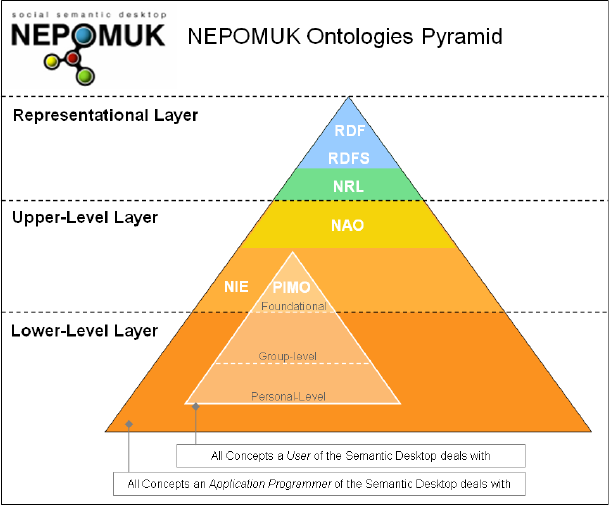
\includegraphics[width=0.8\linewidth]{chapters/background/img/ontologies.png}
\caption{The pyramid of desktop ontologies.}
\label{fig:ontologiespyramid}
\end{figure} 

To accommodate some restrictions specific to describing desktop and personal data, an extension to RDF was developed. It is called NEPOMUK Representational Language (NRL)\footnote{\url{http://oscaf.sourceforge.net/nrl.html}, previously at \url{http://www.semanticdesktop.org/ontologies/nrl}} \cite{Sintek2007}, and is a representational ontology, thus belonging in the top level of the pyramid. It adds Named Graphs and Graph Views to RDF/S and introduces the closed world assumption to the data. The named graphs in NRL are similar to the named graphs defined by \cite{Carroll2005} except that they do not follow the open world assumption. NRL defines graph roles for named graphs, where roles contain information about a graph's data and how it should be handled.

The open world assumption which is usually used on the Web, states that everything that is not known is undefined, which makes sense when working with very large amounts of information, most of it unknown. It does not work as well on the desktop, where we handle personal data that is implicitly known to the user in its entirety. That is why NRL introduces the closed world assumption, which states that everything that is unknown is false. However, NRL does not make any assumptions on the semantics of a graph defined with it. With the use of graph views over named graphs, there can possibly exist different views with different semantics over the same graph.

The upper level ontologies describe basic concepts generalising over multiple domains and activities specific to the desktop and PIM. There are three ontologies in this level: 
\begin{description}
 \item[NEPOMUK Annotation Ontology] (NAO\footnote{\url{http://oscaf.sourceforge.net/nao.html}, previously at \url{http://www.semanticdesktop.org/ontologies/nao/}}) contains concepts which allow users to annotate desktop resources, including custom descriptions, identifiers, tags and ratings. Generic relationships between related resources can be made explicit through properties defined in this ontology.
 \item[NEPOMUK Information Element Ontology] (NIE\footnote{\url{http://oscaf.sourceforge.net/nie.html}, previously at \url{http://www.semanticdesktop.org/ontologies/nie/}}) describes a unified vocabulary for native resources available on the desktop. NIE is in fact a larger framework, where the core part is the NIE ontology, complemented by several smaller vocabularies describing specific types of desktop resources, like files, music, emails, address book contacts, calendar entries, etc. Standards for representating many of these types already existed, either in the form of RFCs or in the form of Web vocabularies. In these cases, the existing resources were used as basis for the respective NEPOMUK ontologies. For example, the NEPOMUK Contact Ontology (NCO\footnote{\url{http://oscaf.sourceforge.net/nco.html}, previously at \url{http://www.semanticdesktop.org/ontologies/nco/}}) was designed based on the VCARD specification (RFC 2426 \cite{RFC2426}), and on the Vcard ontology\footnote{\url{http://www.w3.org/TR/
vcard-rdf/}}, but it has a much broader scope than either of the two. Similarly, the NEPOMUK Calendar Ontology (NCAL\footnote{\url{http://oscaf.sourceforge.net/ncal.html}, previously at \url{http://www.semanticdesktop.org/ontologies/ncal/}}) is an extended adaptation of the W3C calendaring ontology\footnote{\url{http://www.w3.org/2002/12/cal/}}. NIE defines two disjunct classes of resources, \verb|DataObject|s --- the physical representation, and \verb|InformationElement|s --- the interpretation and content of resources. The two are then subclassed in each specific vocabulary of the framework. The NIE classes are designed for machine use in extracting semantic information from existing desktop sources and applications, not for direct handling by the users.
 \item[Personal Information Model Ontology] (PIMO\footnote{\url{http://oscaf.sourceforge.net/pimo.html}, previously at \url{http://www.semanticdesktop.org/ontologies/pimo/}}) is both a upper level ontology and a lower level ontology, as it contains both generic concepts and quite specific ones. From a user's point of view, PIMO is the central ontology of the Semantic Desktop. Its scope is to model the data that the user works with. According to its specification \cite{Sauermann2009a}, ``PIMO is based on the idea that users have a mental model to categorize their environment'', and ``each concept in the environment \dots is represented as [a] Thing in the model''. PIMO defines high level types like Person, Project, Event and Task, which reflect the user's mental image of the objects, not their representation in various desktop applications, nor the files used to store the information about them. That is the task of the NIE ontology and framework, while the PIMO is needed to provide an aggregated view of all 
the possible sources of information about a \emph{thing} the user needs.
\end{description}

The lower level ontologies consist of domain ontologies and application ontologies --- which have very specific or limited use cases. 
Users can import new ontologies into their Semantic Desktop either directly or through applications. When certain ontologies become widely used, it is recommended that they go through a process of standardisation and are included in the desktop ontologies, in order to support reuse. 

Existing ontologies can be customised by users or by application developers, this is however discouraged for the upper level ontologies, as it would affect interoperability between Semantic Desktops.

\subsubsection{The NEPOMUK Reference Implementation}

The reference implementation of NEPOMUK is based on the blueprint defined within the project, but it is not an exact realisation of it. The general structure is maintained however, and several of the possible services are provided. The implementation is done in Java, for portability.

\begin{figure}[tb]
 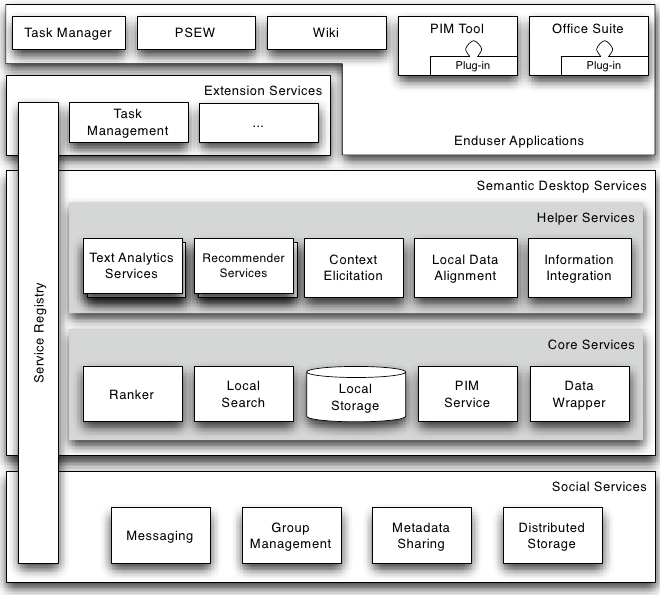
\includegraphics[width=0.8\linewidth]{chapters/background/img/javaarchitecture.png}
\caption{The architecture of the NEPOMUK Java implementation.}
\label{fig:nepomukjava}
\end{figure} 

The service oriented architecture of the Java implementation of NEPOMUK uses SOAP and OSGi for communications between the services, and for discovery. The component which provides the registry and discovery functionality is called the NepomukMiddleware (or Middleware), and it is a service itself. The implementation evolved from a local web server with SOAP, to Eclipse, as it has better support for inter-service communication.

Figure \ref{fig:nepomukjava} \cite{Reif2008} shows the services composing the reference implementation. The core services provide functionalities for extraction, storage, and retrieval of the semantic desktop data. They are fundamental for the functionality of the Semantic Desktop, as they are used by all the other helper services and applications built on top of the framework. 

The storage service is the central service of the Semantic Desktop. All the semantic data is stored and retrieved from here, thus acting as a blackboard (see Section \ref{sub:characteristicsofsd}). The storage service uses existing triple store implementations, current version using Sesame2. Additionally it provides some basic inference and query support. Lucene is used for indexing. 

The DataWrapper service extracts information from desktop sources and stores it in semantic form in the central RDF store. It uses plugins to access and extract data from application specific formats and repositories. Other helper services can be combined with the DataWrapper, to ensure that the data is well integrated and that duplicates are removed (e.g. an integration service), a data alignment service, or an inference service to extract new information based on the existing triples. 

The PIM service provides convenience methods to access and create information in a user's PIMO. 

The local search service provides search functionality over the local repository, supporting both structured queries and full text search. It includes the functionality provided by a Ranker service, which computes resource relevance for better search results. 

Additional helper services were developed: a Context service, Recommender services, Text Analytics services. 
On top of the core services and the helper services, several extension services were developed, to showcase possible uses and to demonstrate how the services can be combined. 
On top of the services, applications were built to provide functionality to the users in a friendly user interface. The interface to this implementation of the NEPOMUK Semantic Desktop is called PSEW (Personal Knowledge Workbench) \cite{Grimnes2009}. It offers a visual way of interacting with the services, as well as several views of the data contained in the local repository. Other specialised applications were developed: a semantic email extension \cite{Scerri2009} to Microsoft Outlook and to Mozilla Thunderbird, a plugin for Microsoft Word \cite{Groza2011} to semantically annotate documents, etc.

The social part of the Social Semantic Desktop was meant to be fully distributed, thus a P2P network implementation was used for the majority of the services. However, a centralised NepomukHub was developed as well, using XMPP. The NepomukHub acts as a server for inter [Semantic] Desktop communication, passing messages between NEPOMUK instances, and also as a shared triple store, where social information, like group memberships, is stored and managed. The messages sent through the NepomukHub transport RDF graphs, thus any semantic information can be shared among desktops. Several social services were developed on top of the P2P network and the NepomukHub infrastructure. They include a Messaging service, a Metadata Sharing service, a Distributed Storage service and Distributed Search. Local services can be extended to use the social services.

\subsubsection{Nepomuk-KDE}

By far the most successful part of the NEPOMUK project was the ``Mandriva Community scenario'' \cite{Lauriere2006} or Nepomuk-KDE\footnote{\url{http://nepomuk.kde.org}} as it became known. It was initially meant as a proof of concept, showing that the blueprint can be realised outside of the reference implementation. The start of the NEPOMUK project coincided roughly with the beginning of development on a new major version of the KDE\footnote{KDE has been rebranded in the mean time to refer to the community instead of the software produced. Thus KDE is no longer an acronym for ``K Desktop Environment''.} Desktop Environment for Linux --- KDE4. Thus it provided the opportunity of including the new research ideas into an emerging platform, more deeply than it could have been done for a system that was already completely designed and implemented. As a result, Nepomuk-KDE is part of the core libraries of KDE and is used in several central applications, the best example being Dolphin, the default file manager. 
Desktop search is also done through NEPOMUK, and metadata creation, such as tagging, rating and commenting, is available desktop-wide. The adoption of NEPOMUK and semantic technologies has been very good, and development on the framework continued after the end of the EU project, driven by the community that was formed.

Including NEPOMUK in KDE also meant convincing the developers of KDE applications to make their software use the new semantic features. It required familiarising them with the semantic technologies used, and encouraging them to participate in the development of the framework and to collaborate on the ontologies. 

For open source projects like KDE, there are restrictions on what libraries can be reused due to software licences. This had an effect in the first stages, on the fact that the Java code of the NEPOMUK reference implementation could not be directly reused. Although it is possible to run Java on Linux, there are restrictions on the distribution of Java libraries. That was one of the reasons why Qt, the language in which KDE is developed, was preferred for Nepomuk-KDE. Although it is possible to use Java libraries in applications, code written in Qt/C++ was preferred by the packagers of the distributions that used KDE4. Thus, despite inferior results and features, many Nepomuk-KDE Semantic Desktops used the Redland\footnote{\url{http://librdf.org/}} C library for the storage service, while at the same time Sesame2 library was available but since it was written in Java, it required additional configuration. Currently Nepomuk-KDE uses a customised trimmed down version of OpenLink's Virtuoso\footnote{\url{http://
virtuoso.openlinksw.com/}}. It is feature-rich, stable, and the close collaboration with the OpenLink developers resulted in a version tailored specifically for running a triple store on a desktop.

Architecture-wise Nepomuk-KDE differs from the blueprint. For simplicity the social part has been ignored in the start, and the focus was on providing easy and simple to use semantic features to attract more contributors before diving into more complex tasks. Several social aspects are being implemented now with the use of NEPOMUK in the Telepathy\footnote{\url{http://telepathy.freedesktop.org/}} project.

The services in Nepomuk-KDE are also different. The preferred inter-service communication method is either through DBus\footnote{\url{http://www.freedesktop.org/wiki/Software/dbus}} or API calls. The services themselves are not defined as Web services running on the desktop, but as KDE modules. They are managed through a NepomukServer service.
As already mentioned, the current implementation of the Storage service uses Virtuoso as the default triple store, although other backends can be configured for use. 
The Data Wrapper function is done by Strigi\footnote{\url{http://strigi.sourceforge.net/}}, but instead of independent plugins for external applications, Strigi is a plugin-based system, with each plugin being responsible for certain types of files. Other exporters of semantic data come from Akonadi\footnote{\url{http://community.kde.org/KDE_PIM/Akonadi}}, the PIM framework of KDE.

The Nepomuk-KDE framework is changing continuously, due to the active community around it. It is evolving together with KDE and because of it, the uptake has been considerable, with many developers adding semantic features to their applications, and thus increasing the visibility and attracting more users.


\subsection{Characteristics of Semantic Desktops}
\label{sub:characteristicsofsd}

\subsubsection{Architecture}
\label{sub:architecture}

Most of the systems described in Section \ref{sec:sdsystems}, along with NEPOMUK, agree on the need for a layered architecture for Semantic Desktops. The layered general architecture shares many common points with the conceptual architecture for applications on the Web of Data, as surveyed in \cite{Heitmann2012}.
It can be divided into three major layers which build on top of each other, with dependencies and even overlaps between them.

\begin{description}
 \item[Data layer] The Semantic Desktop revolves around the [semantic] data that it contains. As such, the architecture is also centred around handling this data. This layer contains the vocabularies for describing the data, and the data itself. 
 \item[Service layer] Based on the data, the Semantic Desktop provides an enabling framework of basic services, which can be either visible or transparent to users. This framework enables the functionalities of the applications. The set of basic services vary among the systems described, but are indispensable to them. These services are central to the desktop, and generally accessible from all applications. Some of the basic services include storage, extraction, integration, query, inference, annotation. 
\begin{description}
 \item[Storage service] can vary from a database system like MS SQL server used by MyLifeBits, to a fully fledged RDF store like Sesame or Virtuoso in Gnowsis and NEPOMUK. Many systems use Jena (SEMEX, IRIS) and some use files. Some use a combination of storage from the options above (MOSE has three --- database, file and Jena RDF store). Depending on the type of storage, semantic resources are identified either by URIs or by unique database IDs. 
 \item[Extraction service] can come under several names --- crawlers, wrappers, gatherers --- however, they provide the same function, that of extracting semantic information from non-semantic sources, whether structured or unstructured. It can vary from simple extractors of metadata already available for files --- like photos (EXIF) and music (ID3), or emails --- sender, subject, to parsing and analysing unstructured text to extract information from multiple file formats (Stuff I've Seen, SEMEX, Gnowsis, NEPOMUK). CALO features natural language analysis to extract entities and relations among them. MOSE also extracts resources and relations from files, and stores two types of information --- R-F links, which specify which resource was extracted from which file, and R-R links, which specify connections between resources. Semantic information extraction plays a significant role in providing the basic functions of a Semantic Desktop, and all the systems described here implement it. The extraction service 
generally comes bundled together with an instance matching service.
 \item[Integration service] (instance matching, entity matching, or de-duplication) has the role of checking if two instances are the same. The definition of \emph{the same} varies from system to system. One of the main uses of this service is complementing the functionality of the extraction service, by checking if a newly extracted entity already exists, in which case, depending on the policies the existing entity is reused instead of creating a copy, or a new entity is created and linked to the existing one.
 \item[Query service] All the systems allow querying their semantic data. Keyword search is supported by IRIS, Semex, Haystack, and MOSE. For keyword search, an \textbf{indexing service} is used, which can be an independent service, or part of the storage or the extraction service. Structured query languages like RDQL and SPARQL are also supported in MOSE, IRIS, Gnowsis, X-COSIM, and NEPOMUK. The ways in which the results are displayed are discussed in the presentation layer. 
 \item[Inference service] Inference on the semantic data is supported by IRIS, Gnowsis and NEPOMUK. This service can be standalone or included in the extraction or the integration service. The quality of the inference results depends on the engine used and the ontologies used to describe the data. 
 \item[Annotation service] All systems allow some type of annotation of resources, however, not always in the form of a standalone service. Annotation refers to creation of metadata for resources, or of new connections between resources. Manual creation of new resources can also be considered annotation. Some automatic annotation is performed by the extraction and the integration services. In Haystack, where there is one access point to the data, the annotation service is in fact a user application, as it happens directly. In MyLifeBits annotations play a central part -- the system allows sharing, annotation of annotations. The most basic types of annotations are tagging and grouping in collections, which are both used for categorisation.
\end{description}
\item[Presentation / Application layer] The user-facing interface of the Semantic Desktop makes up the presentation layer, built on top of the supporting framework. The systems have a large variety of user interfaces, providing functionality that varies from simple resource browsers, to complex PIM tools like email clients and task managers. 
\end{description}

Regarding the applications they provide, the systems are divided in two categories, depending on whether they choose to enhance existing applications with semantic capabilities, or propose new semantically enabled applications to replace existing ones for PIM tasks. X-COSIM, Gnowsis and NEPOMUK belong to the first category, while IRIS and MOSE belong to the second.

The flexible and customisable visualisation of information is one of the distinguishing features of Haystack. It is a Semantic Web browser \cite{Quan2004}, providing a unified interface for the data it contains, with the added functionality of allowing edits \cite{Quan2003b} and customisations. The feature that sets Haystack apart from other semantic browsers is its dynamic creation of user interfaces. This is realised by recursively rendering semantic resources \cite{Huynh2003,Karger2005}. The way an object should be rendered is described in RDF. General visualisations are provided out of the box, but users can customise them according to their needs. 

Most systems provide a resource browser and search interface in the style of Haystack, although usually not as flexible. Some browsers display the underlying ontology. They allow changes to be made to the data directly through this interface. 
Faceted browsing and browsing by association are available in all resource browsers.

MyLifeBits and SEMEX propose that multiple visualisations be supported for resources, depending on the user's context.

\subsubsection{Blackboard and fuzzy layers}

The layers of the architecture can overlap.
The storage service is at the fuzzy border between the data layer and the service layer. It is responsible for the persistent storage of the data and for providing low level access to it. Since the storage service is highly connected with the data, it can be seen as part of the data layer, but at the same time it is a foundational service, and as such it is part of the service layer.

Similarly, services which provide any type of user interfaces are at the border between the service layer and the presentation layer.

Inside the service layer itself we can see a separation based on the level at which the services operate. Some foundation services are more oriented towards the data - like an inference service or the analyser and extractor services. Other services provide more user-oriented functionality, like an annotation service, or a query service. 

Services can use functionality provided by other services, communicating and building on top of each other. The communication between the services, as well as the communication between the services and applications can take several forms: through programming interfaces (APIs provided by the framework), Web standards (Gnowsis promotes a Web server as a desktop service), or P2P communication (MOSE, NEPOMUK).

The architecture of many of the systems uses the Blackboard pattern, where the blackboard is the data storage, or even the entire data layer, which is accessible to all services and applications. They have the role of the specialists in the pattern. The control element is the storage service. Specialists populate the blackboard with data which can then be accessed and refined by other specialists. For example, a PDF extractor service can parse documents and extract titles, authors and affiliations. The data must then be processed by the integration services, so that duplicate authors and affiliations can be merged into a single unique representation. Furthermore, the inference service can then extract co-working relations between the people, based on common affiliations.

\subsubsection{Data Representation}
\label{sub:vocabs}

Semantic data is the most important part of the frameworks, and the way it is described influences the quality and quantity of things that can be done with it.

All the systems define a data model for the data they use and extract. The data models vary from very small and generic, like the one in SEMEX, which has a restricted number of classes and associations, to the comprehensive one provided by X-COSIM.

Being small, SEMEX's ontology is unitary, but the bigger ones usually are modular. MOSE's ontology is divided in small application ontologies belonging to the PIAs and domain ontologies used by the services. CALO also has different ontologies for specific domains and used by specialised agents. X-COSIMO is divided into modules representing different aspects of the data.
More than being modular, the set of ontologies used by NEPOMUK is also layered. The representational level defines the vocabulary used to define the other ontologies. The upper-level ontologies contain domain-independent abstract knowledge. The lower level ontologies contain specialised concrete terms from the user's mental model. The low level PIMO plays an important role in both Gnowsis and NEPOMUK, as it is used to describe the data most often handled by the user.

Most of the frameworks use RDF or OWL ontologies to describe the data.
Only MyLifeBits and SIS do not mention the use of ontologies, MyLifeBits using a flexible database schema to define the data model. 

Another differentiating characteristic is whether or not the data model can be personalised by the users by creating new types and new relations. X-COSIM does not allow the modification of the domain ontology, but it does allow the creation of custom mappings from and to other external ontologies. Haystack and SEMEX on the other hand argue for the need for personalisation of the ontologies by the user, as only in this way, can a truly personal mental model be created. Most systems do support the customisation of the underlying model, as well as the import of new vocabularies in the system, by linking to them or through mappings. This fact raises the challenge of reconciling data described with customised models. 

The long-term study by \cite{Sauermann2008} found that very detailed ontologies are not necessarily more useful for the users, as simpler and more generic relations are preferred over more specific ones. The intuition is that the more precise properties, although better at classification, present the added challenge of choosing the suitable one. 
The same study of using Gnowsis has shown that although customisation of the underlying ontologies is supported, the users only make minimal and rare changes. This result confirms the MyLifeBits hypothesis that although their schema is flexible and can be modified, users will probably not make any changes to it. While a layered system like NEPOMUK's gives more flexibility, allowing users to change and update the ontologies gives too much flexibility for the normal use cases, and would be used only by a few power users, in a very limited number of occasions. Most customisations were sub-classing existing classes and specialising existing properties by creating sub-properties. 


\subsection{Discussion}

In this section we covered some common aspects of the systems regarding their architecture, the functionalities they provide and the way they represent and work with data.
Following again the layered structure used before, we continue with a discussion of some of the shortcomings and possible developments which appear to affect all or most of the Semantic Desktops. 

At the data level, as the systems have evolved, the ontologies they employ have become more complex. While providing good coverage of the PIM domain, comprehensive vocabularies with detailed relationships among types showed that the simpler, more general relations are used much more often, regardless of the possible loss of meaning \cite{Sauermann2008}. Hence, rich ontologies are not necessarily better, since most users prefer simple relations between resources, which are enough to remind them of the connection, without specifying it fully. Detailed vocabularies might prove more useful in the case of automatic processing of data, but using them to manually annotate is costly.

Moving into the service layer, the storage and the indexing services provided by the systems use semantic technologies which have evolved at a rapid pace. A slow repository, and thus slow response times for queries and browsing have at least partially been at fault for the poor uptake of the Semantic Desktops. Fast and memory efficient triple stores are now available.

Regarding the applications provided by the systems, we observed the distinction between integrating semantics into existing applications versus creating new semantic applications. 
Forcing the users to switch from the applications they know to avail of the power of the Semantic Desktop in applications they would need to learn how to use, has not proved to be a successful strategy. However, systems like Gnowsis, X-COSIM and NEPOMUK use plugins to add semantic functionality to existing popular tools, thus letting users continue to use their preferred tools while benefiting from the added semantics.

One of the reasons for the slow uptake of the Semantic Desktop could be the cold start problem, which is observable despite multiple automatic ways of extracting, linking and importing resources, and kick-starting the system. This could prove that the user's manual annotations are more important than the automatically extracted data, which has its own important role though. However, since the automated data comes from sources which are accessible to the user anyway through conventional tools, there is no immediate incentive to use the semantic applications, which translates in little manual information being added into the system, and the benefits delayed further, despite several evaluations \cite{Franz2007,Sauermann2008} proving that Semantic Desktops \emph{are} better for PIM tasks \cite{Franz2009}.

It could also be that the visualisations used for the automatically extracted data are not suitable for the purpose, or not attractive enough.
Generic graph or table visualisations are not appealing, and treating every resource the same is not an effective way of conveying information.

In recent years two developments occurred and influenced the direction in which the Semantic Desktops evolve: \begin{inparaenum}[(i)] \item the exponential growth of semantic data available online, mostly due to the Linked Data initiative and the Linking Open Data project which have a large success, and \item the growing concern about the privacy and security of personal data\end{inparaenum}. 
Some of the information available as Linked Data might be relevant to the users of Semantic Desktops, so using it in applications and services to add value to the users is a low hanging fruit, -waiting to be picked. However, the open aspect of most of the available data causes concern especially when it becomes mixed with valuable private personal information. Privacy is not the only concern, albeit a very important one. Establishing whether the Web information is trustworthy is another concern, and possibly a harder one to tackle.

\section{Conclusion}

This chapter covered Semantic Desktop systems and applications described in literature, starting from the historical ones like the Memex, NLS and Xanadu, to recent ones like NEPOMUK. We showed that they share common goals and characteristics, and we extracted and discussed their general architecture and data representation means. Understanding these is very important for the core part of the thesis, as our work is grounded and builds on top of the framework provided by the Semantic Desktop, specifically, the Nepomuk-KDE Semantic Desktop.

In recent years other systems have emerged, targeting the issues described above, on the desktop or other devices, by using semantic technologies. However, the focus has changed from exploring possible architectures and creating vocabularies, to a more data centric approach. The Semantic Desktop has matured, along with the semantic technologies it employs, so that now new and more exciting, as well as harder, problems arise. Now that the infrastructure has been put in place, the Semantic Desktop awaits the killer app which would bring it and the possibilities it opens into the public eye. Siri\footnote{\url{http://www.apple.com/iphone/features/siri.html}} and Evi\footnote{\url{http://www.evi.com}}, as well as IBM's Watson\footnote{\url{http://www-03.ibm.com/innovation/us/watson/}} have led the way.

In the next part, we continue by presenting the core research of the thesis, which builds on top of the base set by the Semantic Desktop, to better interlink personal information, not only within the desktop, but also to the Web.
